%CONCEITOS---------------------------------------------------------------
\chapter{CONCEITOS}
\label{chap:conceitos}
O presente capítulo abordará os conceitos necessários para uma melhor compreensão dos artifícios utilizados para tratar o problema apresentado no Capítulo \ref{chap:introducao}, assim como uma
explanação sobre os extratores de características de imagens que serão utilizados e o estado da arte atual.

\section{ESPAÇOS MÉTRICOS}
\label{sec:espmet}
Uma métrica em um domínio $\mathbb{S}$ é uma função $d:\mathbb{S}$ $\times$ $\mathbb{S}$ $\rightarrow$ $\mathbb{R^{+}}$ que associa a cada par 
ordenado de elementos ($s_1$, $s_2$) um número real $d$($s_1$,$s_2$) chamado de distância de $s_1$ a $s_2$, e que atenda
as propriedades definidas no espaço métrico\cite{Lima1977}.\par
Um espaço métrico $M$ é um par <$S$, $d$> onde $S$ é um conjunto de elementos e $d$ é uma métrica
(ou função de distância). Esta distância $d$($s_1$,$s_2$) pode ser compreendida como uma medida de dissimilaridade entre dois elementos.
Quanto menor esta distância entre dois elementos, mais semelhantes eles são.
\begin{mydef}
 \label{def:espmet}
  Seja $S$ um conjunto não-vazio de elementos e $d$($s_1$,$s_2$) uma métrica definida sobre $\mathbb{S}$ $\times$ $\mathbb{S}$.
   O par <$S$, $d$> é chamado de espaço métrico desde que $d$ satisfaça as seguintes propriedades:\par
1. $d$($s_1$,$s_1$) = 0 (identidade);\par
2. Se $s_1$ $\neq$ $s_2$ ent\~ao $d$($s_1$,$s_2$) > 0 (n\~ao-negatividade);\par
3. $d$($s_1$,$s_2$) = $d$($s_2$,$s_1$) (simetria);\par
4. $d$($s_1$,$s_3$) $\leq$ $d$($s_1$,$s_2$) + $d$($s_2$,$s_3$) (desigualdade triangular)\\
onde $s_1$, $s_2$, $s_3$ $\in$ $\mathbb{S}$.
\end{mydef}
O conjunto de dados complexos a ser utilizado geralmente apresenta dimensões elevadas, mas também podem não ter dimensão fixa. Para a utilização computacional destes conceitos torna-se necessário o conceito de bola,
empregado em espaços métricos. A seguinte definição é baseada no livro de \cite{Shirali2005}.

\begin{mydef}
 \label{def:bola}
 Seja <$\mathbb{S}$, $d$> um espaço métrico. O conjunto
 \begin{equation}
  S(s_0,r) = {x \in \mathbb{S} : d(s_0, x) \leq r},	onde\ r > 0\ e\ s_0 \in \mathbb{S},
 \end{equation}
  é chamado de bola fechada de raio $r$ e centro em $s_0$. 
\end{mydef}

A aplicação direta das propriedades do espaço métrico neste trabalho reside fortemente na quarta propriedade apresentada pela Definição \ref{def:espmet}. A desigualdade triangular é fundamentada na geometria euclidiana, 
onde a soma do comprimento de dois lados de um triângulo não pode ser superior ao comprimento do terceiro lado, como ilustra a figura \ref{fig:destri}.

\begin{figure}[H]
\centering
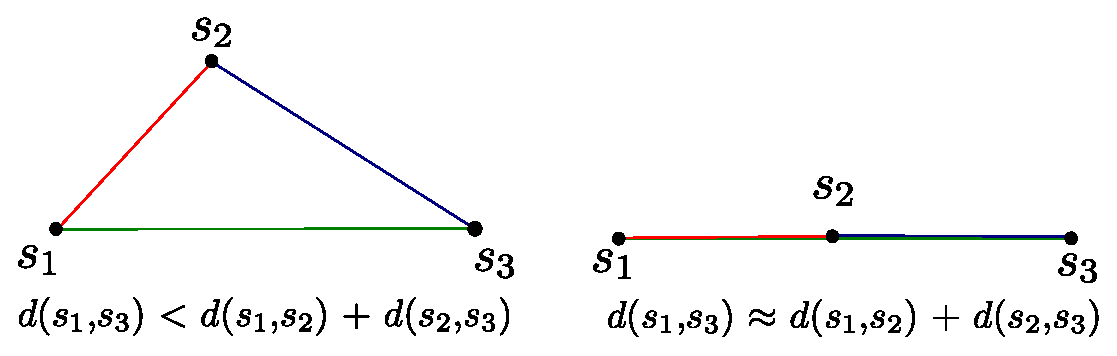
\includegraphics[width=.8\textwidth]{dados/figuras/desig_tri.eps}
\caption{Exemplo geométrico da desigualdade triangular}
\label{fig:destri}
\fonte{Autoria Própria}
\end{figure}

O emprego da desigualdade triangular neste trabalho será detalhado no capítulo \ref{chap:omni}.

\section{FUNÇÕES DE DISTÂNCIA}
\label{sec:funcdist}
Para verificar a similaridade entre dois elementos de um domínio, é utilizada uma função de distância. Esta função recebe como parâmetro um par
de elementos do conjunto e retorna o valor da dissimilaridade entre eles. Quanto mais próximo de zero, mais similares os elementos são.\par

A importância do uso de uma função de distância para este trabalho é fornecer uma métrica de comparação entre os elementos complexos. Além de
necessária para a consulta por similaridade, sua propriedade de desigualdade triangular é utilizada para evitar cálculos desnecessários, fornecendo uma métrica
empregada pela técnica Omni.\par
\subsection{DISTÂNCIA MINKOWSKI}
Dentre as funções de distância, será abordada a métrica Minkowski. Esta métrica é a mais utilizada para cálculos de índice de similaridade
pois é independente da origem do espaço do conjunto de dados, e tem como resultado o valor da dissimilaridade entre dois elementos \cite{Jain1988}.
\begin{mydef}
\label{def:mink}
  Sejam $s_1 = \{s_{11},s_{12},...,s_{1n}\}$ e $s_2 = \{s_{21},s_{22},...,s_{2n}\}$ dois vetores de dimensionalidade $n$ pertencentes ao conjunto de
  elementos $\mathbb{S}$, a distância Minkowski entre esses dois elementos é dada por:
\begin{equation}
		d(s_1,s_2) = \sqrt[p]{\sum_{i=1}^{n}|s_{1i} - s_{2i}|^p}
\end{equation}
\end{mydef}

A figura \ref{fig:minko} ilustra as diferentes formas geométricas geradas de acordo com a métrica $L_p$ utilizada. Para estes determinados valores de $p$, a distância Minkowski recebe nomes
próprios (\textit{distância City-Block} para $p = 1$, \textit{distância Euclidiana} para $p = 2$ e \textit{distância Chebyshev} para $p = \infty$).

\begin{figure}[H]
\centering
\caption{Círculos unitários em espaços bi-dimensionais para diferentes valores de \textit{p}}
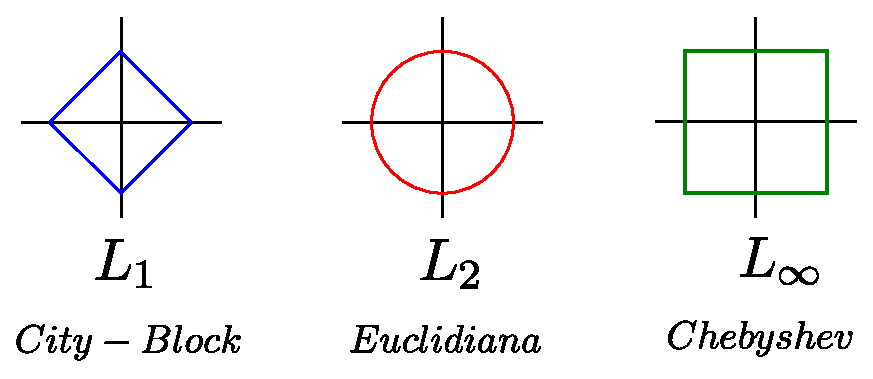
\includegraphics[width=.7\textwidth]{dados/figuras/minko.eps}
\fonte{Autoria Própria}
\label{fig:minko}
\end{figure}

\subsection{DISTÂNCIA CANBERRA}
A distância Minkowski nem sempre é a melhor opção de métrica. A diferença da distância em cada dimensão é elevada
a uma potência $p$ geralmente $\geq 1$  coloca uma enorme ênfase para os casos onde a distância dimensional é grande \cite{Kokare2007}.
Uma alternativa é a distância Canberra. Ela apresenta um cálculo menos custoso do que a distância Minkowski, e atribui um peso
menor para a diferença de distâncias, mas é sensível à origem do espaço de dados.
\begin{mydef}
 \label{def:canb}
 Sejam $s_1 = \{s_{11},s_{12},...,s_{1n}\}$ e $s_2 = \{s_{21},s_{22},...,s_{2n}\}$ dois vetores de dimensionalidade $n$ pertencentes ao conjunto de
  elementos $\mathbb{S}$, a distância Canberra entre esses dois elementos é dada por:
  \begin{equation}
   d(s_1,s_2) = \sum_{i=1}^{n}\frac{|s_{1i} - s_{2i}|}{|s_{1i}| + |s_{2i}|}
  \end{equation}
\end{mydef}


\section{ESTRUTURAS DE INDEXAÇÃO}
\label{sec:index}

Dados complexos costumam apresentar tamanho físico muito elevado quando comparados com dados numéricos ou pequenas cadeias de caracteres, que são os tipos de dados
mais comuns em bancos de dados tradicionais. Para responder consultas que envolvam dados complexos, são necessários mais acessos a disco em relação a uma consulta
que envolva tipos de dados mais simples, como os previamente mencionados. Estes acessos são custosos e precisam ser reduzidos para um melhor desempenho do banco.\par 

Uma maneira de tornar o acesso a disco mais eficiente é evitar movimentar grandes porções do banco de dados do disco para a memória, fazendo o uso de índices dentro do banco de dados. 
Um índice em um SGBDR funciona de maneira semelhante a um índice de um livro. Para procurar um tópico específico, é possível consultar o índice no fim do livro e descobrir qual o número da página
correspondente ao tópico, contornando a necessidade da leitura sequencial do livro até o tópico procurado. Os índices são armazenados em ordem e apresentam um tamanho
muito menor do que um capítulo do livro, reduzindo o esforço necessário para a sua consulta \cite{Silberschatz2011}.\par

Mas índices também podem ser empregados para uso em memória RAM. Enquanto as estruturas de indexação orientadas a disco são armazenadas em disco e apresentam
um custo elevado para serem acessadas, índices orientados a memória estão contidos na memória RAM, assim não existem acessos
a disco para serem minimizados. Assim, uma estrutura de indexação em memória busca reduzir o tempo de computação geral enquanto usa
o mínimo de memória possível. Estas estruturas armazenam ponteiros para as tuplas, que são menos custosos de serem manipulados do que as tuplas \cite{Lehman1986}.\par
				
Dentre as estruturas de indexação em disco para dados tradicionais, destacam-se a B$^{+}$-Tree e índices bitmap. Para indexação em memória,
podem ser utilizadas estruturas como B-Trees e arrays para preservar a ordenação natural dos dados, enquanto estruturas de hashing
(\textit{Chained Bucket Hashing, Linear Hashing e Extendible Hashing}) aleatorizam os dados dentro do índice.

\section{EXTRATORES DE CARACTERÍSTICAS}
\label{sec:extcarac}
O principal foco deste trabalho é o emprego destas técnicas para bases de dados constituídas por imagens. Para isto, torna-se necessário o uso de uma miríade de extratores de características
das imagens, para um maior refinamento do uso de consultas por similaridade. Estas características podem se referir a: atributos visuais (cor, forma, textura), atributos lógicos (identificação
de elementos) e atributos semânticos (identificação de emoções humanas).\par

As características visuais podem ser utilizadas como histogramas de cores para a análise de cor, matrizes de co-ocorrência para a análise de textura e
métodos baseados em contorno para a análise de forma. Geralmente, consultas são feitas utilizando uma combinação destas características, e não apenas uma delas.\par

Dado uma palheta discreta de cores definida por alguns eixos de cor, o histograma de cores é obtido através da discretização das cores da imagem e contagem
do número de vezes que cada cor discreta ocorre na matriz da imagem \cite{Swain1991}. As vantagens do uso do histograma de cores é a sua simplicidade computacional e pouca
sensibilidade a alterações na imagem (rotação e translação), particularmente útil para a representação de objetos tridimensionais. Entretanto, duas imagens completamente 
diferentes podem apresentar o mesmo histograma de cores.\par

Para a análise de textura, o objetivo e conseguir distinguir regiões que apresentam cores similares (como folhagem e grama), analisando o padrão
de variação dessas cores. A técnica mais utilizada analisa conjunto de pares de pixels da imagem em tons de cinza e monta estruturas com informações características.
A principal estrutura utilizada nesta técnica é a "Matriz de co-ocorrência", e a sua utilização é a identificação de padrões
em uma imagem, sendo considerada crucial para pesquisas por similaridade em imagens médicas \cite{Glatard2004}.\par
												
Diversas medidas que podem ser extraídas pela análise de textura estão presentes no trabalho de \cite{Haralick1973}. Algumas das métricas extraídas
da análise das matrizes de co-ocorrência são  relacionadas com características específicas da textura da imagem como homogeneidade, contraste
e a presença de estruturas organizadas dentro da imagem. Outras métricas caracterizam a complexidade e a natureza das transições dos tons de cinza presentes
na imagem, como a entropia.\par

Os extratores de características das imagens utilizados neste trabalho são do framework Arboretum, desenvolvido pelo Grupo de Bases de Dados e Imagens (GBDI) da Universidade de São Paulo - campus São Carlos.


